\chapter{Methods}
% have to mention about the ability of working on only one sample
% somewhere here...

The method of tackling this problem will be based on previous research done in this domain. There are three essential components for this project:
\begin{figure}[h]
\caption{Basic flowchart}
\centering
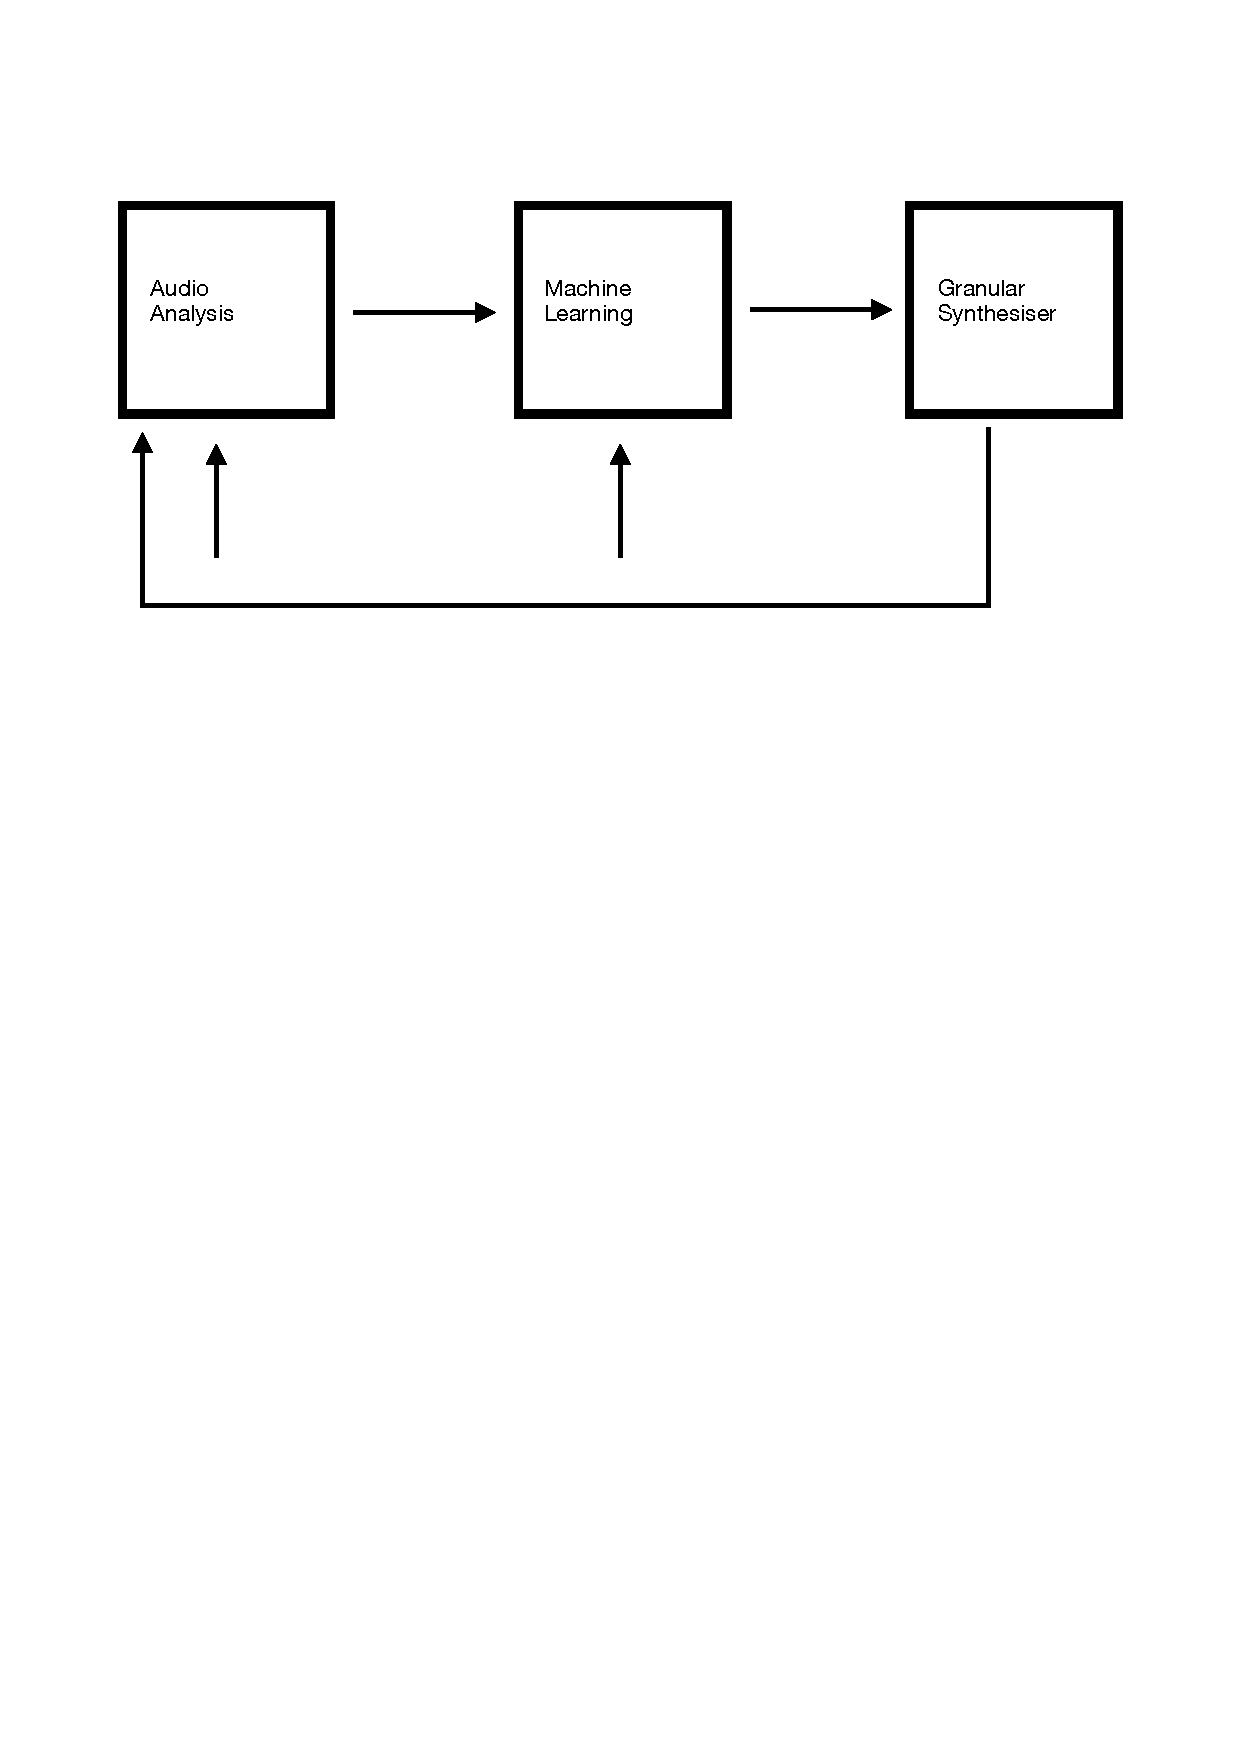
\includegraphics[width=0.5\textwidth]{images/flowchart}
\end{figure}

The box ``Granular Synthesiser'' in figure 1. represents a granular synthesizer.
It was implemented in C++, using the `JUCE' framework (SOURCE). (Add about it being
quasi-synchronous, and all other possible information.)

`Machine Learning' stands for the predictions module, or more
precisely the Multilayer Perceptron model built in `Keras', and later
ported to C++ with the help of the `Frugally Deep' library.

Lastly, the `Audio Analysis' square represents the aspect of the
project responsible for extracting audio features from input
sounds. This was done with the `Essentia' library, that allowed me to
perform frame cutting, windowing, extracting the spectrum and finally
MFCCs on any specified buffer.

\section{Audio descriptors}
\subsection{Definitions and Formulation}

As mentioned in \autoref{chap:lit} the MFCC algorithm is proven to be
one of the most reliable desriptors available, and can not only
describe the temporal qualities, but also be indicative of the changes
that happen in the input signal. (source again?) Therefore, it is the
only algorithm used, with further justifications for this decision
provided later in this chapter.

The Mel-frequency cepstrum is a representaion of the short-term power
spectrum of sound, based on a linear cosine transform of a log power
spectrum on a nonlinear mel scale of frequency (WTF, CHANGE AND ADD
SOME REFERENCE TO THE DESCRIPTION). In turn, the MFCCs, are
coefficients that collectively make up the Mel Cepstrum. The biggest
advantage of this algorithm is that in the MFC the frequencies are
spaced in a way which approximates the human auditory system more
closely than the cepstrum used in a Fourier Transform. 

The MFCCs are commonly derived as follows:

\begin{enumerate}
\item{Take the Fourier Transform of a signal}
\item{Map the powers of the spectrum obtained into the mel scale,
    using triangular overlapping windows}
\item{Take the logs of the powers at each of the mel frequencies}
\item{Take the discrete cosine transform of the list of mel log
    powers, as if it were a signal}
  \item{The MFCCs are the amplitudes of the resulting spectrum}
\end{enumerate}

There can be variations on this process, such as differences in the
shape or spacing of the windows used to map the scale, or addition of
dynamics features such as delta and deltadelta coefficients.(ADD
SOURCE AND CHANGE - total ripoff)

In order to achieve  usable (source, what if we took mfccs on the
entire song lol?) results from the algorithm, often the first element
of the list above is done on a windowed frame of an input signal.

Let's assume, that we are trying to analyse an audio input which is 10
seconds long. In order to obtain usable results, we have to separate
the input into multiple excerpts, and compute the algorithm on each of
these frames. In order to `smooth' out the values and achieve better
results (more specific, maths, studies) the frames are often
overlapped, so that certain `history' of is taken into account. And
information in one frame is not treated as independent of the rest of
the signal. This is often reffered to as `hopsize'. The effect of this
behaviour is that consequtive frames are overlapped. Lengths of both
the frames, and the size of the hopsize vary, adn depend on
application. However the standard values are assumed to be 2048
samples and 1024 samples consequtively. With these values our input
would be split into frames of size 2048 (approximately x ms.), and
would take one frame, analyse it, and move 1024 samples ahead, to
start the analysis of the next frame.

For each frame, MFCC are calculated based on the extracted
FFTs. The result for one frame is a vector of 13 floating point
values, each corresponding to a different range of frequencies.

At a sampling rate of 44.1kHz, and a buffer size of 512 samples, this
corresponds to exactly 45 vectors of 13 float values for one second of
sound. Meaning that our hypothetical sound of length of 10 second
would comporomise of 450 MFCCs.

Several different audio features have been experimented with,
especially in the quest of finding universal ones, that could be
applied to any source file in the granular synthesizer. One of such
features is onset detection. It's implementation consists of the
spectral flux algorithm, thresholding and peak finding, in order to
estimate how many peaks, or onsets are in a specified buffer. (more
description, or is this useless to talk about?)

However, during testing, which is described in chapter 4, such a
connection was not found, therefore this project solely depends on MFCCs.

\subsection{Implementation}
\subsubsection{Essentia}

The process decribed above was achieved with algorithms provided by
the `Essentia' library\cite{noauthor_homepage_nodate}. It works in a
modular way, that can roughly be described as spiltting the algorithms
into lower, and higher level algorithms. They can be then `stacked' to
create more complex chains of computation, capable of extracting, as
in this case, the MFCCs.

% maybe fuck around and create a graph here?
The process is as follows:

\begin{itemize}
\item Firstly, an audio buffer on which the computation will be
  performed has to be specified. Here, one second of sound is written
  into a buffer (C++ vector), that then gets passed to the first algorithm
\item `FrameCutter' is where the buffer first arrives. This function
  splits the buffer into multiple frames, as dictated by the
  parameters. Then, each frame, separately is sent further down the
  chain, with the help of a while loop
\item Each consequtive frame of the buffer arrives at the `Windowing'
  algorithm, which essentialy smoothes out the edges of each frame.
\item Once the windowing is applied to the frame, the spectrum of the
  input signal is calculated.
\item Finally, the Mel-Frequency Cepstrum Coefficients are calculated
  for the frame
\end{itemize}

\begin{figure}[!h]
\caption{logic of the MFCC computation}
\centering
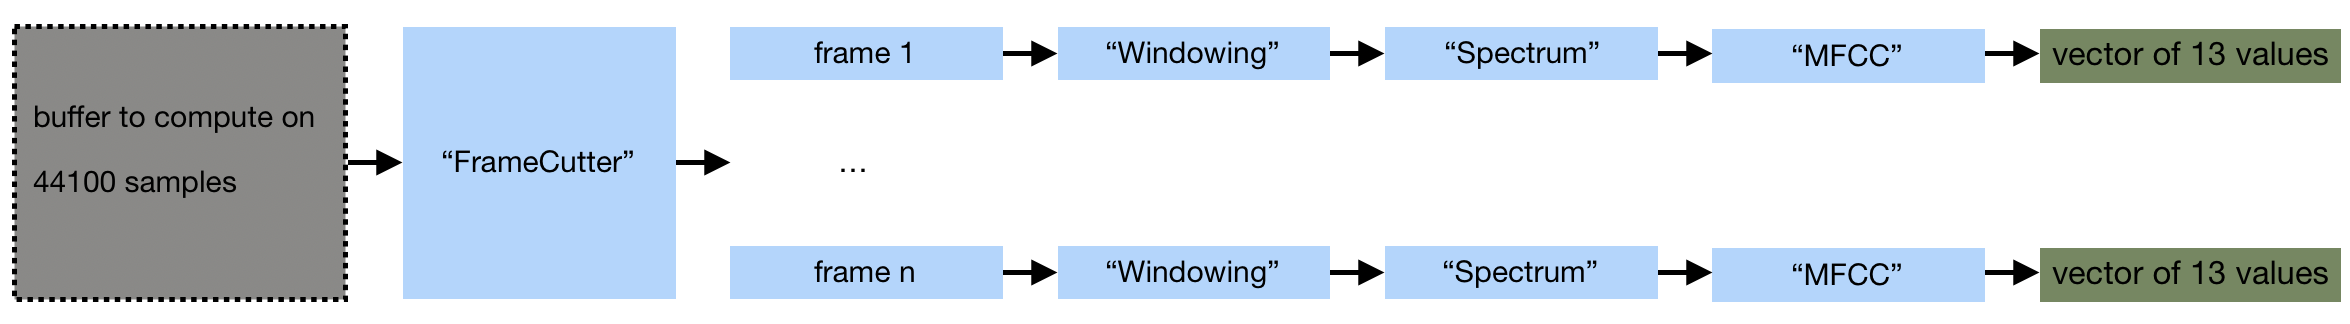
\includegraphics[width=1\textwidth]{images/essentia_logic}
\end{figure}

Code responsible for creation of the buffer:
\begin{figure}[!h]
\caption{filling the buffer}
\centering
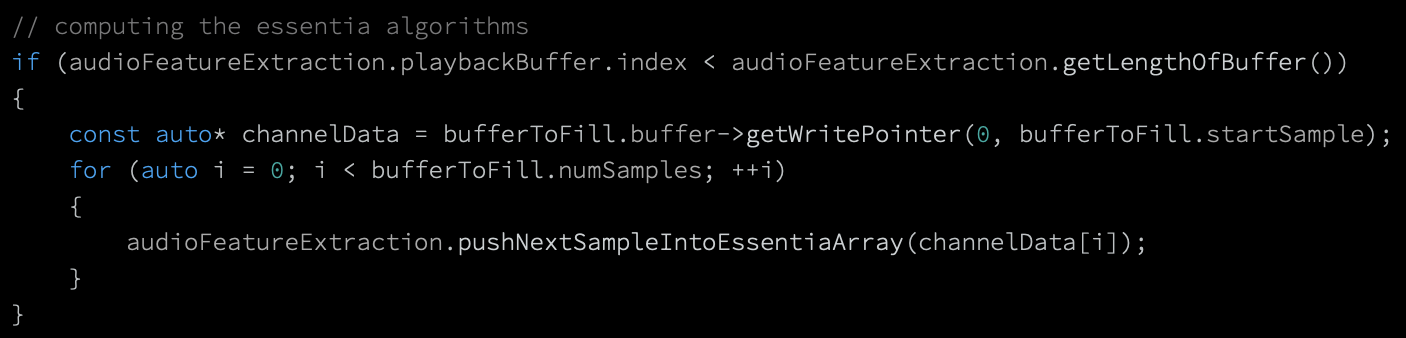
\includegraphics[width=0.8\textwidth]{images/essentia_buffer}
\end{figure}

This process is repeated for each frame, which at the sampling rate of
44.1kHz, and a buffer size of 512 samples, with frame size of 1024,
and hopsize of 512 samples equals to exactly 45 frames per
second. Which in C++ code looks as follows:
\begin{figure}[!h]
\caption{computing Essentia algorithms}
\centering
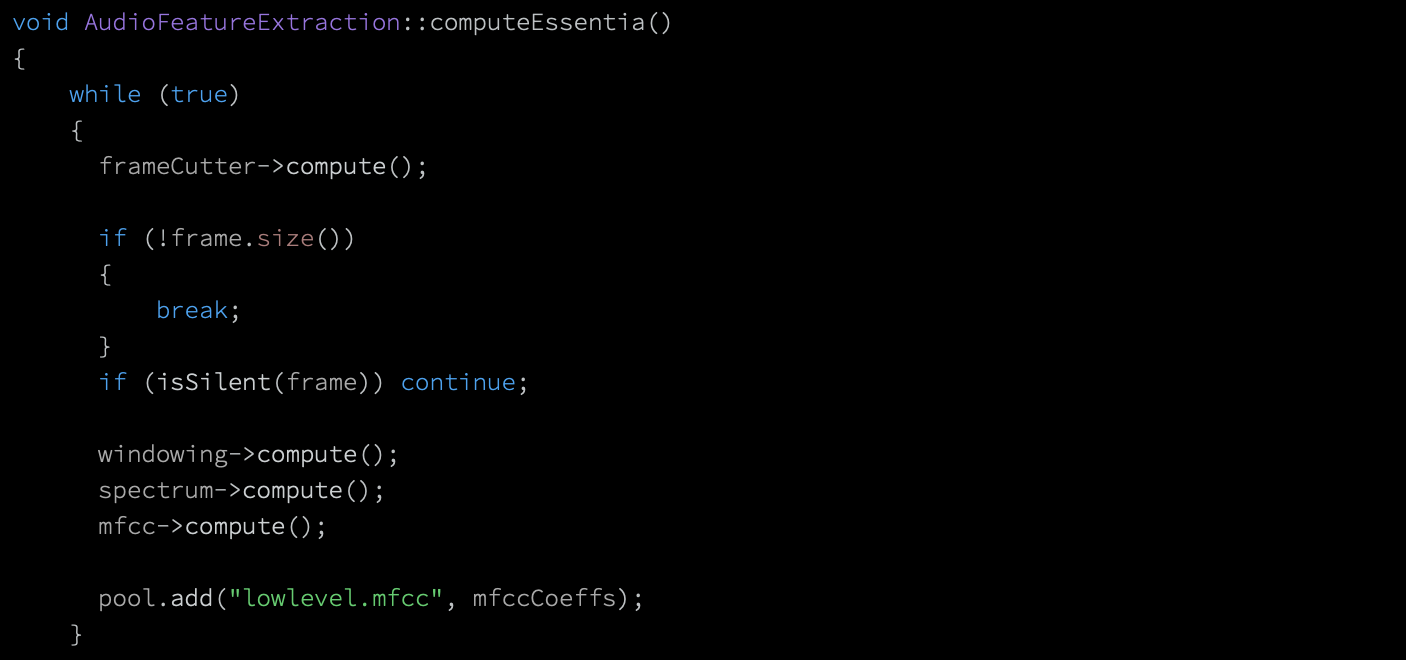
\includegraphics[width=0.8\textwidth]{images/essentia_algorithms}
\end{figure}

\section{Predictions}
\subsection{Dataset}
\subsubsection{Definitions and Formulations}
% everything done on one sample only -> here?
A dataset, linking the MFCC values with the synthesis parameters had
to be created, in order to create a way to use the information, and
make a coorelation between parameters, and audio
descriptors. Initially, I have set out to create a data set of every
possible combination of parameter values, and their corresponding
MFCCs. However, even though there are only 5 adjustable parameters,
with a static hop size of a tenth of each parameter, it would take
more than 1000 hours to complete this task, given that each parameter
combination would be sampled for exactly one second.

In order to avoid this limitation, a different approach was
taken. Every second, each parameter was set to a random value between
their unique minimum and maximum values. Consequently, the audio
features were extracted on each of these iterations, for exactly 10000
instances, which allowed for a creation of a dataset, of 10000
different parameter values, each corresponding to a 2D vector, of
size 45 by 13 containing the computed MFCCs. (source here, where
did i get the idea?)

\begin{figure}[!h]
\caption{Example of one instance of the dataset}
\centering
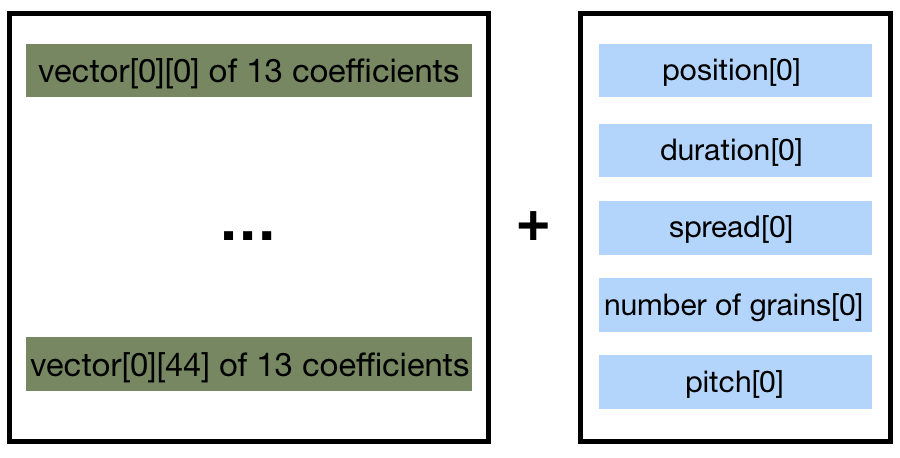
\includegraphics[width=0.8\textwidth]{images/dataset_example}
\end{figure}

\subsubsection{Implementation}

Creation of the dataset was done inside of the C++ JUCE
synthesis code. A function responsible for setting a random value for
the parameters was implemented using the JUCE::Random class. After
each, 1 second long iteration, the class instance is giving a random
value between specified ranges, different for each parameter, which
results in independent changes. This function is a pseudorandom number
generator, for which seed was not specified, in order to get different
values, if multiple datasets were desired.

After the parameter values are overriden by this function, the MFCC
computation is initialised for a buffer, with the sound resulting from
previously set parameters.

Then, two arrays are created, which contain the audio analysis
results, and parameter values. In order to conveniently export these
results as .JSON files, the arrays are appended to a `Pool' data
structure from the `Essentia' library. `Pool' includes an elegant
solution for saving it's contents into a .JSON file with the help of
`YamlOutput' function, like so:

\begin{lstlisting}
  mergedMFCCs = factory.create("YamlOutput",
                                  "filename", "MFCC.json",
                                  "format", "json",
                                  "writeVersion", false);
  mergedMFCCs->input("pool").set(mergePool);

  mergePool.merge(pool, "append");
\end{lstlisting}

The resulting dataset is imported into a Python script, in order to
perform the training of different predictive models.
% add example JSON output of one frame and maybe a diagram of structure

\subsection{Neural networks}
\subsubsection{Multilayered Perceptron}

% add diagram of structure of the MLP as well code snippets
% add bit about scaling in the c++ part
% revise this, add more specific things - why this architecture, how
% was this tested? show some results here, or in the next section?
% add specific values in the paragraph about how many epochs
% etc... look at python code for this!!!!!!!!!

Many different algorithms were considered for the task of predicting
parameters, given the MFCC values (examples). Due to the success of
neural networks for this task (source), other options were
disregarded. There are many different possibilities when it comes to
the architectures and types of networks, and it was shown that a
Multilayered Perceptron, as well as Long-Short Term Memory network are
both viable choices, with Bidirectional LSTMs having the best
performance (check if true, and quote the infamous paper).

Due to time constraints, as well as the lack of computational power on
machines I had access to, only a feedforward, 3 layer Multilayered
Perceptron network was implemented. The popular `Keras' (source?)
library was used to create the architecture in Python.

The only activation function used was `ReLu'. The `Adam' optimizer,
with mean absolute error served as the optimization function.

Before the data was fed to the network, it was scaled between 0 and 1,
using the MaxMinScalar form the sklearn library.

The 45 by 13 MFCC vectors served as the features, and a vector of 5
different parameter values as the output of the network.

The 2D MFCC vectors, were flattened, consequently making the first
layer of the MLP having 585 perceptrons. The second layer has 20
inputs, and the third 15.

The last layer has 5 ouputs - one for each parameter to be predicted,
and as this is a regression problem - no activation function.

The network was trained for X epochs, making use of an early stopping
function, to prevent overfitting. The loss function values for training
set is about 0.9 and test set 0.12.

Different approaches were considered for handling the communication
between the C++ synthesis code, and Python machine learning
code. During the first few iterations of the project, starting with
the first prototype, OSC messages were used to send audio analysis
values to Python, predict parameters there, and send the predictions
back to C++. This process however, was not optimal. It was relatively
slow, not efficient, and required two separate programs to be running
in order to give basic functionality.

Therefore, later in the production a search for a better solution was
done. I have found the `Frugally Deep' library that seemed to resolve all the
issues present at the time. It required a Keras model to be saved into
a .JSON file, and then it would convert it into XXX and allow for
usage of the model directly in the C++ code, with a fairly
straightforward way. 

Consequently, the model in Keras was saved after training with like so:
%CODE

With the toolset supplied by the `Frugally Deep' library, it was then
converted into XXX like so:
%CODE

As seen above, with the file converted, only a few lines of code were
needed to make use of the model directly in the C++ synthesis program,
creating a standalone application, silmultaniously allowing for much
quicker and simpler performance, without the need of any additional
software running.

\section{Synthesis}

\subsection{Granular Synthesis (basic explenation of the granular synth concept)}

Describing granular synthesis in one paragraph is impossible
without cutting some edges, and leaving out many intricacies of the
technique. However, a summary of sorts, describing the main concepts
behind the algorithm will be attempted here. 

Granular synthesis was first imagined by Xenakis and Gabor (cite
microsound and figure out more about it from there) in the late
1960s. It was a breakthrough technique, that was as controversial as
it was inspiring back then. It was mostly achieved manually, cutting
tape and sticking it back together. A very slow, and labour intesive
process.

The most basic granular synthesiser requires some sort of an envelope
over the grain, grain waveform, whether generated by an oscillator or
taken from a sampled audio, and some grain spatialization. (get the
graph from microsound and describe it basically.) 

It is an extremely versatile method of synthesis, capable of
generating anything between pitched sounds, similar to an additive,
fm, or subtractive synths, to segmentation techniques, all dependent
on 3 main parameters. Grain envelope, grain waveform, and grain
length.

%Grain clouds...
%Xenakis...
%Rodes...
%Some other folks...
%graphs, graphs, graphs and pictures...

\subsection{The JUCE implementation (author's implementation)}

An original implementation of a granular synthesiser was done in order
to gain the ability of creating a standalone program, with all the
functionality mentioned in CHAPTER 1, and achieve all of the project's
objectives. A possibility of creating only the audio analysis and
machine learning modules existed, with the use of an external
synthesiser, however that approach would obviously not allow for a
creation of `all in one' application, as stated in CHAPTER 1.

Separate, original implementation of the sythesizer allowed for the other
modules to be included inside of it, therefore making the entire
program independent.

The `JUCE' (source) library was used as the fundament of the
synthesizer.  It is one of the most established libraries in the
professional audio community, being used by companies such as `Cycling
74', and `Korg' amog others (cite website?). On top of all things
audio, it provides a convenient way of creating a graphical user
interface, which was an important part of this project. Thanks to
`JUCE', the implementation was kept minimal, and elegant.

% how it is build
The core of the implementation is contained in one class
`GrainStream'. All the functionality for one grain, as well as the
stream, otherwise vector of grains is contained in it.

Even though the concept of granular sythesis is very difficult, the
implementation here is kept fairly minimal, to restiric the amount of
dimensions, reducing learning time for the neural networks, and
consequently minimizing the time needed to create an appropriately
sized dataset.

In reponse to these requirements only 6 adjustable parameters were
implemented.

\subsubsection{Loading of samples}

Loading of samples is implemented with the function setAudioSource
like so:
\begin{lstlisting}
  void GrainStream::setAudioSource(AudioFormatReader& newAudioFile)
  {
    int length = static_cast<int>(newAudioFile.lengthInSamples);

    //update grain parameters
    this->fileSize = length;
    this->samplingRate = static_cast<int>(newAudioFile.sampleRate);

    //clear the audio source and read new WAV
    this->AudioSourceBuffer.reset(new
                                     AudioSampleBuffer(newAudioFile.numChannels, length));
    newAudioFile.read(this->AudioSourceBuffer.get(), 0, length, 0,
                        true, true);
  }
\end{lstlisting}

It is using the JUCE::AudioFormatReader and JUCE::AudioSourceBuffer
classes to handle this behaviour. The length of the sample, as well as
it's sampling rate are also read here, and used to update global
values. 

\subsubsection{Grain creation}

Grains are created by feeding the buffer values
from the input sample into the a vector of floats that makes up one
grain.
%put int the entire createGrain function???????

% what parameters are being manipulated
% how each parameter influences the output sound
% describe each function and add snippets!
\subsubsection{Position}
The position of each grain is determined by the `FilePos' dial. It's
value serves as a parameter to the `setFilePosition' function, which
in turn `communicates' the starting position for each grain with the
use of `filePosition' integer. It was required to subtract 1 from the
dial's value, because...XXX

The following code is responsible for
this task:

\begin{lstlisting}
  void GrainStream::setFilePosition(int startingSample)
  {
    this->filePosition = startingSample - 1;
  }
\end{lstlisting}

\subsubsection{Grain Size}
The size of each grain varies between the minimum of 10ms and maximum
of 1 second. It can be easily set using the Grain Size GUI dial. Value
of the dial serves as a parameter to the `setDuration' function:
\begin{lstlisting}
  void GrainStream::setDuration(int duration)
  {
    //update duration and compute sampleDelta
    this->durationOfStream = duration;
    this->sampleDelta = static_cast<int>(this->samplingDelta *
    (duration/1000.0f));

    for (oneGrain grain : grains)
    {
      grain.grainDataEndPosition = grain.grainDataEndPosition +
      this->sampleDelta;

      if (grain.grainDataEndPosition >= this->fileSize)
          grain.grainDataEndPosition = (this->fileSize - 1);
    }
  }
\end{lstlisting}

It is responsible for computing the end position of each grain
(grainDataEndPosition), with the use of a `sampleDelta'
variable. Which means the difference between the starting and ending
position of a grain. The end position is then calculated by simply
adding the delta to the start position.

Simple but effective error handling is then implemented, by ensuring
that the end position of a grain will never be bigger than the length
of the sample.

\subsubsection{Spread}
The so called spread functionality could be summarized as randomizing
the starting position of one grain, independently of the others, in a
certain range.

Let's assume that the FilePos dial is set to 10000 samples, which
would correspond to approximately 4 seconds into the file, assuming a
samapling rate of 44,1kH (maybe note somewhere, that whenever I talk
about sampling rate this assumption is made, sounds
proffessional). With the `spread' dial turned down to 0, each
consequtive grain would start at exactly 10000 samples, play for it's
duration, and die, creating space for another grain to be spawned,
again at the starting position of 1000 samples.

Once the dial has a value bigger than 0, a random number generator is
used, to create a random integer in the range of original file
position - value of the dial, and original file position + value of
the dial. The random number is created for each new grain,
consequently creating a new position for each new grain.

To illustrate that with an example, turning the dial to the value of
100 would create a new, random starting position for each grain in the
range of 9900 - 11000, assuming our original file position was 10000,
as in the example above.

This allows for each grain to have independent starting positions,
creating a more interesting clusters, that do not sound so repetative
and static.

Above described functionality is implemented like so:

%change, add code
\begin{lstlisting}
if (filePositionOffset == 0 || (this->filePosition -
filePositionOffset) <=0)
grain.grainDataStartPosition = this->filePosition;
\end{lstlisting}

Where `filePositionOffset is the value of the dial.
% add code beneath
\subsubsection{Number of active grains}
There can be up to 10 grains, meaning that the 2D vector of
grains can contain up to 10 vectors. The main struct of one grain
looks like this:

and the 2D vector like this:

\begin{itemize}
\item Adding grains

Adding grains to the stream is done by simply adding a grain vector to
the 2D vector containing all the grains -> the stream of grains. In
code referenced as `grains'.

\item Removing grains

Conversly, the removal of grains is done in exactly the same way, only
using `pop\_back' rather than `push\_back', and simply removing howver
many vectors (grains) indicated by the dial. 

\item Control over the stream of grains

One function is implemented in order to decide whether the user wants
to add, or remove grains from the main stream like so:
\end{itemize}
% CODE

Because of this, the interaction is kept quite simple, and the size
can be decided with the use of only one dial. If the value of the dial
if bigger than current size of the stream, we remove grains to match
the value. Conversly, if the dial value is smaller, we add grains to
the 2D vector `grains'.

\subsubsection{Pitch}
Each grain, as defined in the `OneGrain' struct defined above, has a
variable called grainDataPitchScalar, responsible for changing the
pitch of grains independently. In the spirit of simplicity, however,
in this perticular implementation, the pitch scalar is kept global,
with the possibility of extension.

It is binded to the Pitch dial visible in the GUI, which changes the
`pitchOffsetForOneGrain' variable, which is then sent to the :

% CODE

% this part of the code is probably fucked up hahahhaahahahahahha :(
The grain.grainDataPitchScalar can therefore only have values between
THIS and THAT, consequently either speeding up or slowing down the
playback of each grain, and affecting the pitch.

\subsubsection{Global gain}
The global gain of the signal is simply controlled by the globalGain
variable, which is used for scaling each individual sample sent to the
audio buffer like so:

\begin{lstlisting}
  sample *= static_cast<float>(globalGain)
\end{lstlisting}

The globalGain variable is directly controlled with the global gain
dial in the GUI.

\subsubsection{Sound output}

The sound output is mostly handled by the JUCE library, with the use
of the provided `getNextAudioBlock' function. The audio block, or
buffer is being filled with samples determined in the Grain class,
more specifically, in the `createGrain' function contained within that
class:

%code here

All the functionality needed to determine all the previously mentioned
parameters is  here. What is being returned is samples, one by one
with which to fill both channels of the buffer.

% (where do the grains come from)(how does the
% behaviour change depending on the sample)

%maybe add stuff from microsound about the parameters, and how they
%influence the sound.
%
%also, maybe add how the personal preference for the granular sound
%influenced this area of production.

%What belongs in the "methods" section of a scientific paper?
%
%    Information to allow the reader to assess the believability of your results.
%    Information needed by another researcher to replicate your experiment.
%    Description of your materials, procedure, theory.
%    Calculations, technique, procedure, equipment, and calibration plots. 
%    Limitations, assumptions, and range of validity.
%    Desciption of your analystical methods, including reference to any specialized statistical software. 
%
%The methods section should answering the following questions and caveats: 
%
%    Could one accurately replicate the study (for example, all of the optional and adjustable parameters on any sensors or instruments that were used to acquire the data)?
%    Could another researcher accurately find and reoccupy the sampling stations or track lines?
%    Is there enough information provided about any instruments used so that a functionally equivalent instrument could be used to repeat the experiment?
%    If the data are in the public domain, could another researcher lay his or her hands on the identical data set?
%    Could one replicate any laboratory analyses that were used? 
%    Could one replicate any statistical analyses?
%    Could another researcher approximately replicate the key algorithms of any computer software?
%
%Citations in this section should be limited to data sources and references of where to find more complete descriptions of procedures.
%Do not include descriptions of results. 


%%% Local Variables:
%%% mode: latex
%%% TeX-master: "dissertation"
%%% End:
